\chapter{Related Works} \label{bg}
Machine learning is an exceedingly vital tool in modern society. Nonetheless, as the issues which machine learning endeavours to resolve become more intricate, the possibility of utilizing a single centralized intelligence diminishes. One possible remedy to this problem is the distribution of both data and computation amongst multiple nodes. Transitioning from centralized approaches to decentralized approaches also offers numerous advantages. For example, it has been proven mathematically that the accuracy of a distributed system surpasses that of a centralized one \cite{swarmbetterthanone}. The following sections will provide an overview of some of the state-of-the-art approaches used to distribute machine learning amongst multiple nodes.

\section{Federated Learning}
% Introduce federated learning
Federated Learning (FL) \cite{survey_on_fed_learning} is a technique in machine learning that aims to train a single model using all available data across nodes without requiring any data to be shared among them. \\

% Intro on how fed learning works and different types
There are a multitude of published FL frameworks \cite{fed_table_survey}, each with different merits and drawbacks for certain use cases. Federated Averaging (FedAvg) \cite{fed_learning} is a commonly used yet simple framework, which splits training into iterations where three steps take place:
\begin{enumerate}
	\item A copy of the current model is sent to each node from the central server.
	\item Each node performs some training with their copy of the model and their own private data.
	\item The trained models from each node are sent back to the server to aggregate into the new server model.
\end{enumerate}
The server model is improved over time, beyond what could be achieved by simply training on a the data stored on a single node. \\

% Specify why federated learning is better than conventional learning
As it does not require data to be shared between nodes, FL is naturally beneficial for privacy sensitive tasks compared to conventional machine learning where the data is aggregated in a central location \cite{fed_privacy}. Additionally, as FL performs training on multiple nodes in parallel, it can make better use of available training resources in situations where processing power is not only distributed among multiple nodes but also limited on each node, such as Internet of Things (IoT) \cite{fed_iot_2}.

% federate distributed
FL has given rise to several variations that eliminate the need for a single central server. One such variant is Multi-Center Federated Learning \cite{multi_center_fed_learning}, which involves multiple central servers, each connected to different clusters of nodes. Another approach is to use leader election to select a node to function as the server \cite{fed_leaderelec}. This method can improve network resilience because, if the server fails, a new server is elected. However, leader election becomes a complicated problem in sparsely connected networks of nodes, resulting in a significant increase in overhead \cite{leaderelec_car}.

\section{Blockchain} \label{bg:bc}
% Breif intro of what a blockcahin is
Blockchain technology enables a network of nodes to record transactions on a shared ledger in a fully decentralized manner \cite{blockchain_review}. In a conventional blockchain, any participating node is permitted to add a transaction to the ledger, but once a transaction is executed, it becomes immutable and irreversible. Although blockchains are primarily associated with cryptocurrency and financial transactions, any type of data, including neural network weights, can be recorded as a transaction.

% Disadvantages of using blockchain
When a blockchain is scaled up, it may encounter performance issues. For instance, the Bitcoin network typically processes only 7 transactions per second on average \cite{blockchain_scale}. High confirmation delay and performance inefficiency are two primary issues related to this paper when scaling up a blockchain \cite{blockchain_scale}. These issues could prove catastrophic in a system like a swarm of robots, where it is crucial to always have the latest data and optimize limited processing power.

\section{Swarm Learning}
% Introduce swarm learning
Swarm Learning (SL) is a subcategory of FL which operates in a completely distributed and decentralised manner. SL enables the collaboration of nodes to learn a shared global model, however in contrast to FL, a central server is never used. SL also does not use leader election, so all nodes on the network are given the same importance.

In SL, the model on which new training is performed is known as the global model. However, unlike FL where the global model is stored in a central location, the global model in SL does not materially exist, but is instead a concept which is agreed upon by the nodes in the network.

\begin{figure}[h]
	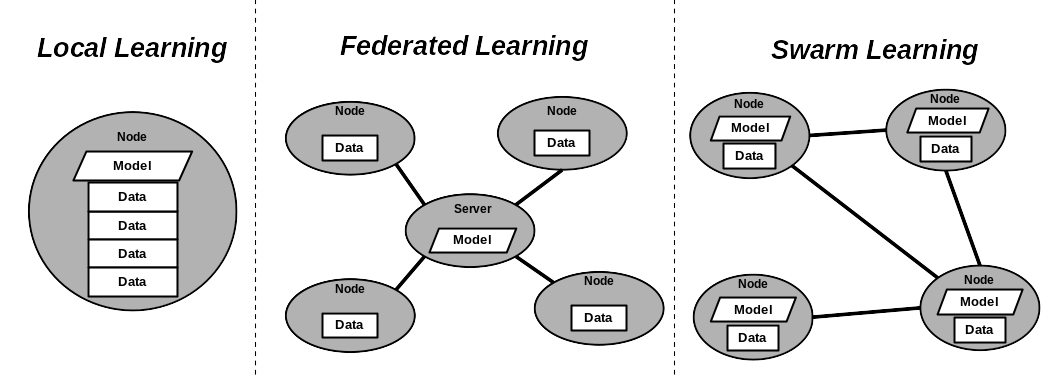
\includegraphics[width=\linewidth]{fedvsswarm}
	\caption{Diagram of different learning algorithms. Each \emph{Node} indicates a single training machine, and each line denotes a connection between two machines, along which the model can be shared. In the swarm learning diagram, the dashed lines show that each local model is an approximation of the global model.} \label{fig_learning}
\end{figure}

One SL algorithm, referred to by this paper as SwarmBC, uses a blockchain to store the global model \cite{swarm_learning}. In this version of SL, training is performed by repeating the following steps:
\begin{enumerate}
	\item A node obtains a copy of the global model from the blockchain.
	\item The node performs some training with their copy of the model and their own private data.
	\item The updated model is merged with the latest blockchain model and sent back to the blockchain for other nodes to use.
\end{enumerate}

% Specify why swarm learning is better than conventional learning or federated learning
SL exhibits many of the same benefits of FL over conventional learning, but it also improves upon FL in some aspects. As is often the case when comparing decentralised algorithms to their centralised counterparts \cite{swarm_resil}, the absence of a central server theoretically makes SL more resilient and robust to failures than centralized FL approaches such as FedAvg. The absence of a central server in SL not only means that the system does not entirely rely on a single node, but also that it is less sensitive to disruptions in connections between nodes. In FL, if a connection between two nodes ceases to exist, the node can no longer participate in learning without some form of tunnelling. In contrast, in SL, even if a connection between two nodes is lost, the two connected nodes are still likely to be connected to other operational nodes, enabling the system to continue functioning normally.

The utilization of FL with leader election effectively addresses the challenge of ensuring system robustness, as it enables any node to serve as a replacement for the server in the event of network disconnection. Nevertheless, it is important to note that a swarm of nodes is not often completely interconnected, and the connections between the nodes are often subject to changes. This dynamic and sparse network topology can present significant complexities when it comes to leader election, leading to an increase in overhead \cite{leaderelection}. The lack of a leader election process in SL makes it a more viable option in such situations.

Finally, a swarm of nodes can offer greater scalability compared to its centralized counterpart, particularly if agents are restricted to communicating with only their nearby neighbours \cite{swarmscalable}. This is primarily because in such cases, there is no need for all communications to travel to a single node or server that may not be able to handle the significant volume of traffic. In a swarm, where nodes are limited to a certain number of close neighbours, the size of the swarm becomes less significant, since a single node would not experience a difference between a small or large swarm, as it would have the same number of neighbours. Consequently, SL is typically more scalable than FL.